\documentclass[conference]{IEEEtran}
\IEEEoverridecommandlockouts
\usepackage{cite}
\usepackage{amsmath,amssymb}
\usepackage{graphicx}
\usepackage{booktabs}
\usepackage{array}
\usepackage{xcolor}
\usepackage{textcomp}
\usepackage{url}

% Red marker for anything that still needs a real measurement or a fact only the authors know.
% Search for "TODO" before submission: there must be none left.
\newcommand{\todo}[1]{{\color{red}\textbf{[TODO: #1]}}}

\begin{document}

\title{Dictionary Loading and Lookup Optimizations for a Paradigm-Based Kannada Morphological Analyzer: A Same-Hardware Ubuntu and Windows Evaluation}

\author{
\IEEEauthorblockN{Aryan K Shetty, Siddharth Prabhu, Aniketh Nishikanth Shetty}
\IEEEauthorblockA{Department of Computer Science and Engineering\\
Manipal Institute of Technology, MAHE, Manipal -- 576 104, India}
\and
\IEEEauthorblockN{Ashwath Rao B, Ph.D.}
\IEEEauthorblockA{School of Computer Engineering\\
Manipal Institute of Technology, MAHE, Manipal -- 576 104, India}
}

\maketitle

\begin{abstract}
Paradigm-based morphological analyzers describe inflection through paradigm classes and finite-state suffix transitions, and are widely used for Indian languages. We study the run time of the paradigm-based Kannada morphological analyzer developed at MIT Manipal in the Discourse Integrated Dravidian Language -- Dravidian Language Machine Translation (DIDL-DL MT) project, funded by the Ministry of Electronics and Information Technology (MeitY). Following the project guide, we evaluate (i)~removing non-essential regular expressions, (ii)~binary search over a sorted dictionary, and (iii)~multicore processing, on one laptop that dual-boots Ubuntu 24.04 and Windows~10, with confidence intervals from repeated runs. Timed as a whole program on 100 words, the optimized analyzer is 12.4 times faster than the original on Ubuntu (95\% CI 12.2--12.5) and 18.3 times faster on Windows (17.6--19.0), with byte-identical output; the dictionary loader contributes only a small part of this. A pre-processed dictionary shortens load-and-lookup time by 2.5 to 10 times, but with loading excluded binary search is 20 to 36 times slower than a hash look-up, so the gain comes from pre-processing and not from the search. Running several analyzer processes in parallel speeds up batches of 5,000 words by up to 2.2 times on Ubuntu and 2.8 times on Windows, whereas parallelising only the dictionary look-ups is slower than serial.
\end{abstract}

\begin{IEEEkeywords}
paradigm-based morphological analyzer, Kannada, DIDL-DL MT, dictionary lookup, binary search, Storable, MCE, benchmarking
\end{IEEEkeywords}

\section{Introduction}
Kannada, like the other Dravidian languages, is agglutinative: a root combines with a chain of suffixes that carry case, tense, aspect and agreement. A morphological analyzer is therefore an early component of any machine translation pipeline for these languages. Paradigm-based analyzers handle the variety of inflection by grouping roots into paradigm classes, that is, sets of words that take the same suffixes, and by recording the allowed suffix sequences of each class in a finite-state automaton (FSA).

This paper concerns the paradigm-based Kannada morphological analyzer built at Manipal Institute of Technology within the DIDL-DL MT project, funded by MeitY, Government of India. The analyzer is a Perl program that reads three resources at start-up: a lexicon of roots written in WX notation~\cite{bharati1995,gupta2010}, an FSA transition table, and an allomorph mapping file. Reading the lexicon is repeated every time the program is started, and the lexicon keeps growing as new paradigms and word classes are added.

The project guide suggested three ways to make the analyzer faster: remove regular expressions that are not needed for simple string matching, replace hash look-up by binary search over a sorted dictionary, and use several CPU cores. We evaluate each suggestion under controlled conditions. Our contributions are:
\begin{itemize}
\item a same-hardware comparison of Ubuntu and Windows, with run counts, confidence intervals and an explicit statement of what each experiment does and does not measure;
\item whole-program and multicore measurements on the analyzer itself, not only on its dictionary look-ups;
\item evidence that the gain usually credited to binary search comes from pre-processing the dictionary, not from the search step;
\item a correctness check showing that the optimized analyzer reproduces the original output byte for byte;
\item scripts and raw data that allow every number in this paper to be regenerated: \todo{repository URL}.
\end{itemize}

\section{Related Work}
Paradigm-based analysis has been applied to many Indian languages. Bapat et al.~\cite{bapat2010} combine a paradigm-based inflectional system with finite-state machines for Marathi. Motlani et al.~\cite{motlani2016} build a free finite-state analyzer for Sindhi in which a paradigm lists all word forms and features of a stem. For Kannada, Antony et al.~\cite{antony2010} present a paradigm-based analyzer that uses sequence labelling with support vector machines and report 96.25\% accuracy on verbs. Forsberg and Ranta~\cite{forsberg2004} express inflection paradigms as functions in a functional programming language, and Beesley and Karttunen~\cite{beesley2003} give the standard account of finite-state morphology. In the papers we reviewed, the emphasis is on coverage and accuracy; run-time engineering of the analyzer receives little space. Our work addresses that side for the DIDL-DL MT analyzer. For the tools we use, Storable serialises Perl data structures to a binary file~\cite{storable}, and MCE is a many-core engine for Perl that distributes work over worker processes~\cite{mce}.

\section{The Paradigm-Based Analyzer}
\textbf{Lexicon.} \texttt{dict\_all.txt} has 105,696 lines and 98,038 distinct roots. Each line holds a root, its category, its paradigm class, gender and number, for example \texttt{mara,N,1,n,3sg,}. Roots are written in WX notation.

\textbf{FSA.} \texttt{dfsa\_270526.txt} has 13,270 lines of the form \emph{from-state, to-state, suffix\_sandhi\_tag} and contains 3,361 distinct suffix strings. An input word is analysed by stripping candidate suffixes from its end, looking up the remaining stem, and accepting the parse if the paradigm class of the stem has a transition at the state reached by the stripped suffixes.

\textbf{Allomorph file.} \texttt{alloMorphMappingFile.txt} is empty in the release we received, so no allomorph rules were applied in any experiment reported here.

\textbf{Processing.} The main loop reads one token at a time and passes it through a chain of tests (punctuation, symbols, numerals, then dictionary and FSA analysis). It is sequential; no part of the analysis is distributed over cores. In the original code, the suffix test inside the analysis builds a pattern from the candidate suffix at run time (\texttt{\$word =~ /\$suffix\$/}), and the program writes about 264--271~KB of debugging output to \texttt{STDERR} for 100 words.

\section{Experimental Setup}
\subsection{Platform and software}
All runs used one HP ProBook 450 G9 that dual-boots Ubuntu and Windows (Table~\ref{tab:env}). Windows was measured under both its Balanced and High-performance power plans; Ubuntu was measured after setting the CPU governor to \texttt{performance}. Because the power setting changes absolute times considerably (Section~\ref{sec:cross}), the primary comparison pairs Ubuntu with Windows High performance.

\begin{table}[t]
\caption{Test environment (same physical machine).}
\label{tab:env}
\centering\small
\begin{tabular}{@{}p{0.27\columnwidth}p{0.67\columnwidth}@{}}
\toprule
Device & HP ProBook 450 15.6-inch G9 \\
CPU & 12th Gen Intel Core i5-1235U \\
Memory & 8 GB (7.64 GB usable), 3200 MHz \\
Storage & WD Green SN350, 1 TB SSD \\
Ubuntu & 24.04.4 LTS, kernel 7.0.0-38-generic; Perl 5.38.2 (system); MCE 1.889; Storable 3.32; governor \texttt{performance} \\
Windows & 10 Pro 22H2, build 19045.6466; Perl 5.42.2 (MSWin32-x64-multi-thread) in the later session, version of the earlier P1, P2, B1 session not recorded; MCE 1.904; plan High performance (and Balanced); Defender real-time protection on \\
Power state & Ubuntu: AC connected, load average 0.54 at the start of the session of 23 October 2026. Windows: AC connected, session of 1 November 2026. \\
\bottomrule
\end{tabular}
\end{table}

\subsection{Data and procedure}
The lexicon and FSA are the same files on both systems (SHA-256 identical after line-ending normalisation). The test set is the 100-word list supplied by the project guide; all 100 entries are lexicon entries, 13 of them multi-word. Each timed run starts from nothing: it reloads the dictionary from disk (from the operating system's file cache) and then looks up the 100 words. Reported times therefore include loading. Three experiments were run:
\begin{itemize}
\item \textbf{P1} (5 runs): the original loader, which applies five regular-expression operations per line, against a loader that uses \texttt{tr}, \texttt{index} and a limited \texttt{split}. Both build the full value hash and the gender map, and the script checks that their contents are identical.
\item \textbf{P2} (5 runs): a regex-free hash loader against a pre-built sorted file searched by binary search. Both hold the full dictionary values, which are compared for equality.
\item \textbf{B1} (10 runs): a regex-free hash of root words, a Storable cache of that set, a sorted file of root words with binary search, and MCE with four workers over chunks of 25 words.
\end{itemize}
In P1 and P2 the two methods alternate within each run in a fixed order (baseline first); in B1 the four methods are run as consecutive blocks. Each experiment has its own baseline, so speed-ups are comparable only within an experiment.

Three further experiments were run in later sessions (Ubuntu on 23 October, Windows on 1 November 2026) with the same scripts and run counts, under the High-performance plan on Windows. \textbf{E} (end to end): the original and the optimized analyzer are timed as complete programs on the 100 words, 31 runs per condition with alternating order and the first run as a pre-declared warm-up; in the \emph{quiet} condition the standard error of both programs is discarded, in the \emph{as distributed} condition the original writes its debugging output to a file. \textbf{L} (look-up only): the dictionary is loaded once, outside the timer, into a hash and into a sorted array; 100, $10^4$ and $10^6$ queries (90\% roots, 10\% guaranteed misses, fixed seed) are timed with 10, 10 and 5 runs, alternating the order of the two methods. \textbf{PAR} (parallel analyzer): a batch of 100, 1000 or 5000 words is split into contiguous chunks, MCE starts one complete analyzer process per chunk (1, 2, 4 or 8 processes, 10 runs each), and the chunk outputs are joined in the original order. Because every process has its own interpreter, the analyzer's global variables are never shared. Batches larger than 100 words repeat the 100-word list.

The binary search is the procedure given by the project guide: set $\text{low}=0$ and $\text{high}=n-1$; while $\text{low}\le\text{high}$, let $\text{mid}=\lfloor(\text{low}+\text{high})/2\rfloor$; return true if the word equals entry \text{mid}; set $\text{high}=\text{mid}-1$ if the word is smaller and $\text{low}=\text{mid}+1$ otherwise; return false. For 98,038 roots at most $\lceil\log_2 98038\rceil=17$ comparisons are needed.

\subsection{Statistics and correctness check}
Every recorded run is included, except the pre-declared warm-up run of experiment E. We report the mean with a 95\% Student-$t$ interval, the speed-up as the ratio of means, and a 95\% interval for the speed-up from a percentile bootstrap (10,000 resamples; in E whole runs are resampled, so the two programs of a run stay paired). All values are recomputed from the raw per-run files by a script in the repository. As a correctness check, the original and optimized analyzers were run on the 100 words; their outputs are byte-identical and non-empty on both systems, and identical across systems after line-ending normalisation. The 3,361 suffix strings contain no regular-expression metacharacters, so replacing the run-time pattern by a \texttt{substr} comparison is semantically equivalent for this FSA.

\begin{table*}[t]
\caption{Results (ms, mean with 95\% interval in brackets; speed-up with 95\% bootstrap interval in parentheses). Ubuntu 24.04, \texttt{performance} governor, against Windows 10, High-performance plan, on the same laptop. All runs included. Speed-ups are relative to the baseline of the same experiment.}
\label{tab:results}
\centering\small
\begin{tabular}{@{}lcccc@{}}
\toprule
 & \multicolumn{2}{c}{Ubuntu 24.04} & \multicolumn{2}{c}{Windows 10 (High perf.)} \\
\cmidrule(lr){2-3}\cmidrule(lr){4-5}
Method & Time [95\% CI] & Speed-up & Time [95\% CI] & Speed-up \\
\midrule
\multicolumn{5}{l}{\textit{P1: original vs.\ regex-free loader (5 runs)}} \\
\quad Original loader & 140 [123--158] & 1 (base) & 529 [326--733] & 1 (base) \\
\quad Regex-free loader & 122 [120--125] & 1.15 (1.08--1.25) & 418 [229--607] & 1.26 (0.86--1.81) \\
\midrule
\multicolumn{5}{l}{\textit{P2: hash vs.\ sorted file + binary search, full values (5 runs)}} \\
\quad Hash (regex-free load) & 124 [120--129] & 1 (base) & 383 [359--407] & 1 (base) \\
\quad Sorted file + binary search & 49.2 [47.7--50.7] & 2.52 (2.45--2.60) & 103 [91.4--115] & 3.71 (3.40--4.00) \\
\midrule
\multicolumn{5}{l}{\textit{B1: root-word set (10 runs)}} \\
\quad Hash (regex-free load) & 63.0 [62.3--63.7] & 1 (base) & 256 [246--266] & 1 (base) \\
\quad Storable cache & 15.6 [14.6--16.7] & 4.03 (3.83--4.27) & 25.5 [23.3--27.6] & 10.06 (9.30--10.79) \\
\quad Sorted file + binary search & 11.2 [10.7--11.7] & 5.60 (5.39--5.81) & 30.5 [27.6--33.4] & 8.40 (7.68--9.05) \\
\quad MCE, 4 workers & 146 [144--148] & 0.43 (0.43--0.44) & 553 [524--581] & 0.46 (0.44--0.49) \\
\bottomrule
\end{tabular}

\end{table*}

\section{Results and Discussion}
\subsection{Removing regular expressions from the loader}
On Ubuntu the regex-free loader reduced the loader time from 140.5 to 122.5~ms, a speed-up of 1.15$\times$ (95\% CI 1.08--1.25), or 12.8\% less time (Table~\ref{tab:results}). On Windows the interval includes 1: 1.26$\times$ (0.86--1.81) under High performance and 1.07$\times$ (0.82--1.40) under Balanced. The Windows runs vary strongly (coefficients of variation of 21--36\% with only five runs), so no effect can be claimed there. Removing regular expressions from the loader is therefore a small and, on Windows, unconfirmed gain; its effect on the analyzer as a whole is a separate question (Section~\ref{sec:e2e}).

\subsection{Pre-processed dictionary and binary search}
Both pre-processed workflows are clearly faster than the corresponding hash baseline on both systems, and every interval excludes 1 (Table~\ref{tab:results}). Against the full-value hash of P2, sorted file plus binary search is 2.52$\times$ faster on Ubuntu and 3.71$\times$ faster on Windows. In B1, the Storable cache is 4.03$\times$ (Ubuntu) and 10.06$\times$ (Windows) faster, and the sorted file with binary search is 5.60$\times$ and 8.40$\times$ faster. Which of the two is faster reverses between the systems: the sorted file wins on Ubuntu (11.2 against 15.6~ms), the Storable cache on Windows (25.5 against 30.5~ms).

These results should not be read as binary search beating hashing. A hash look-up is a constant-time operation, and in our experiments the time is dominated by loading. The sorted file is read line by line into an array without regular expressions or hash construction, and the Storable file restores a finished hash; both avoid the per-line parsing and hash building that the baseline repeats. The measurements show the value of a pre-processed dictionary, not of the search algorithm. We therefore isolated the search step (experiment L). On Ubuntu a hash look-up took about 75--93~ns per query and binary search about 2.1~$\mu$s, so binary search was 23$\times$ slower at $10^4$ queries (95\% CI 18--30) and 29$\times$ slower at $10^6$ queries (26--31); the 100-query timings are close to the timer resolution and are not interpreted. In Perl a hash look-up is one built-in operation, whereas the binary search is an interpreted loop of about 17 iterations, so the ratio may differ in a compiled language. On Windows a hash look-up took 110--163~ns and binary search 3.3--3.9~$\mu$s, which is 20$\times$ slower at $10^4$ queries (95\% CI 15.8--27.5) and 36$\times$ slower at $10^6$ queries (32.9--41.2). Over both systems binary search was thus 20 to 36 times slower than the hash.

\subsection{Multicore lookup with MCE}
With four MCE workers the lookup of 100 words was slower than the serial baseline on both systems: 0.43$\times$ on Ubuntu (95\% CI 0.43--0.44) and 0.46$\times$ on Windows (0.44--0.49); under the Balanced plan it was 0.83$\times$ (0.72--0.93). The 100 hash look-ups take well under a millisecond in total, while starting and coordinating four worker processes costs tens to hundreds of milliseconds. This experiment parallelises only dictionary look-ups. It does not speed up, and cannot show the benefit of, parallel morphological analysis, because the analyzer's own loop remains sequential. A fair multicore test must run the analyzer itself on a batch of words. Because the analyzer keeps its dictionary and state in global variables, the simplest safe design is to split the batch into contiguous chunks, run one complete analyzer process per chunk, and join the outputs in the original order; each process then has private state. We ran this design with MCE (experiment PAR, Table~\ref{tab:par}); in every configuration the joined output was identical to the serial output. On Ubuntu, two processes gave 1.80$\times$ (95\% CI 1.77--1.83) on 5,000 words, four gave 2.05$\times$ (1.89--2.21) and eight gave 2.22$\times$ (2.11--2.31), which are parallel efficiencies of 90\%, 51\% and 28\%. For 100 words the gains were small (1.32$\times$ with two processes, 1.06$\times$ with eight), because every process must reload the dictionary. From the one-process times, the analysis costs about 3.2~ms per word plus a fixed start-up of about 0.17~s. The gain therefore saturates well below the number of processes. We did not isolate the cause; a plausible one is that the i5-1235U is a hybrid, low-power mobile CPU whose cores cannot all run at full speed under load, but this is untested. On Windows, two, four and eight processes gave 1.88$\times$ (95\% CI 1.72--2.06), 2.29$\times$ (2.10--2.50) and 2.81$\times$ (2.57--3.07) on 5,000 words (efficiencies 94\%, 57\% and 35\%). For 100 words, parallel execution helped little with two processes (1.11$\times$) and was slower than one process with four (0.74$\times$) and eight (0.54$\times$), so batches that small should not be parallelised (Fig.~\ref{fig:par}). The one-process Windows times varied more (coefficients of variation of 12--15\% for 1,000 and 5,000 words) than the parallel ones, which widens the intervals.


\begin{table}[t]
\caption{Parallel analyzer (experiment PAR): wall-clock time in seconds for the whole batch (mean of 10 runs) and, in parentheses, the speed-up over one process. Words per batch in the first column.}
\label{tab:par}
\centering\footnotesize
\begin{tabular}{@{}rcccc@{}}
\toprule
 & 1 process & 2 processes & 4 processes & 8 processes \\
\midrule
\multicolumn{5}{l}{\textit{Ubuntu}} \\
\quad 100 & 0.52 & 0.40 (1.32$\times$) & 0.43 (1.23$\times$) & 0.49 (1.06$\times$) \\
\quad 1000 & 3.40 & 1.90 (1.78$\times$) & 1.68 (2.03$\times$) & 1.83 (1.86$\times$) \\
\quad 5000 & 16.31 & 9.08 (1.80$\times$) & 7.95 (2.05$\times$) & 7.35 (2.22$\times$) \\
\midrule
\multicolumn{5}{l}{\textit{Windows}} \\
\quad 100 & 0.90 & 0.81 (1.11$\times$) & 1.22 (0.74$\times$) & 1.68 (0.54$\times$) \\
\quad 1000 & 5.07 & 3.49 (1.45$\times$) & 3.27 (1.55$\times$) & 3.28 (1.54$\times$) \\
\quad 5000 & 24.71 & 13.12 (1.88$\times$) & 10.81 (2.29$\times$) & 8.81 (2.81$\times$) \\
\bottomrule
\end{tabular}
\end{table}

\begin{figure}[t]
\centering
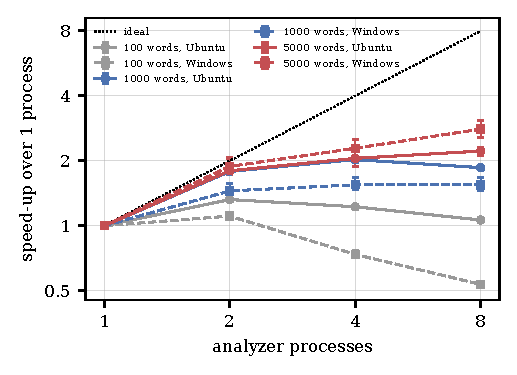
\includegraphics[width=\columnwidth]{parallel_scaling.pdf}
\caption{Speed-up of the parallel analyzer over one process (log scales; whiskers show the 95\% bootstrap interval). Solid lines: Ubuntu; dashed lines: Windows; dotted line: ideal scaling.}
\label{fig:par}
\end{figure}

\subsection{Cross-platform comparison}\label{sec:cross}
Speed-ups have the same direction on both systems, but absolute times differ. Under like-for-like power settings, Windows took 1.6 to 4.1 times as long as Ubuntu depending on the method. The power plan alone matters: switching Windows from Balanced to High performance reduced the P1 baseline from 864.6 to 529.1~ms. We did not test other explanations, such as differences between the two Perl builds (5.38.2 on Ubuntu, 5.42.2 on Windows in the later session), the file systems, or antivirus activity (Windows Defender real-time protection was on). For this reason we compare speed-ups within a system and absolute times only under matching power settings (Fig.~\ref{fig:speedups}). The newer experiments show the same pattern. The whole-program speed-up is larger on Windows (18.3$\times$ against 12.4$\times$), but the Perl versions differ, so the difference cannot be attributed to the operating system alone. In absolute terms the optimized analyzer needed 1.02~s on Windows against 0.51~s on Ubuntu, and the original 18.7~s against 6.3~s (quiet condition).

\begin{figure}[t]
\centering
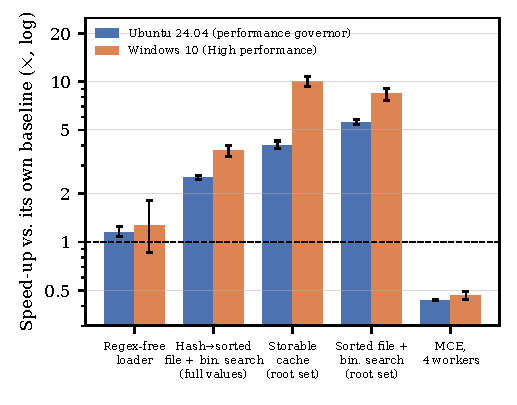
\includegraphics[width=\columnwidth]{speedups.pdf}
\caption{Speed-up over the baseline of the same experiment (log scale; bars show the mean ratio, whiskers the 95\% bootstrap interval). The dashed line marks no change.}
\label{fig:speedups}
\end{figure}

\subsection{End-to-end analyzer timing}\label{sec:e2e}
None of the three experiments above times the analyzer itself, so experiment E times both complete programs on the 100 words (30 timed runs per condition after the warm-up). On Ubuntu the optimized program is 12.36$\times$ faster in the quiet condition (95\% CI 12.17--12.54) and 12.63$\times$ faster as distributed (12.55--12.70); on Windows the factors are 18.31$\times$ (17.59--19.01) and 16.83$\times$ (15.68--17.96), Table~\ref{tab:e2e}. The order of execution had no visible effect on Ubuntu (12.40$\times$ when the original ran first, 12.32$\times$ when the optimized ran first) and a small one on Windows (18.7$\times$ against 18.0$\times$ in the quiet condition, 16.4$\times$ against 17.3$\times$ as distributed). Including the warm-up run does not materially change any result. The Windows timings varied more (coefficients of variation of 8--19\%).

The optimized file differs from the original in three ways: the suffix test in the analysis loop, where a pattern built at run time from every candidate suffix is replaced by a \texttt{substr} comparison; 21 debugging \texttt{print} statements that are commented out; and a rewritten dictionary loader. According to P1 the loader change is worth only about 18~ms per run, 0.3\% of the 5.8~s saved, so the speed-up comes from the first two changes. This experiment does not separate them: \todo{ablation: original with only the suffix test replaced, and original with only the debugging output removed}. The optimized file also uses \texttt{builtin::trim} and therefore needs Perl 5.36 or later.

\begin{table}[t]
\caption{End-to-end analyzer time for 100 words (ms, mean of 30 timed runs; speed-up with 95\% bootstrap interval).}
\label{tab:e2e}
\centering\footnotesize
\begin{tabular}{@{}llccc@{}}
\toprule
System & Condition & Original & Optimized & Speed-up \\
\midrule
Ubuntu & quiet & 6326 & 512 & 12.36 (12.17--12.54) \\
Ubuntu & as distributed & 6238 & 494 & 12.63 (12.55--12.70) \\
Windows & quiet & 18723 & 1023 & 18.31 (17.59--19.01) \\
Windows & as distributed & 19235 & 1143 & 16.83 (15.68--17.96) \\
\bottomrule
\end{tabular}
\end{table}

\subsection{Threats to validity}
(1)~Times include loading from the operating system's file cache, so disk speed is not measured. (2)~In B1 the methods run in blocks, and in P1 and P2 the baseline always runs first, so drift and cache effects are not fully balanced. (3)~P1 and P2 have only five runs, which leaves wide intervals on Windows. (4)~Each experiment has its own baseline, and B1 stores only root existence, not the paradigm values the analyzer needs. (5)~All 100 test words are lexicon entries, so look-ups of unknown words are not measured, and 13 entries contain spaces. (6)~One laptop with a hybrid-core CPU was used, and thermal state was not recorded on either system, and the Perl version of the earlier Windows session (P1, P2, B1) was not recorded. (7)~An earlier Ubuntu session ran with the \texttt{powersave} governor and was discarded; it was not archived. (8)~The allomorph file was empty, so that stage of the analyzer was not exercised. (9)~Experiments E, L and PAR were run in one Ubuntu session (23 October 2026) and one Windows session (1 November 2026), separately from P1, P2 and B1, which were run earlier. (10)~Equivalence of the two analyzers was checked on the 100 test words only; the optimized loader also skips lines whose root field is empty, which the original keeps. (11)~Larger batches in PAR repeat the same 100 words. (12)~The speed-up in E is that of a bundle of three changes, not of regular-expression removal alone. (13)~The two later sessions used different Perl versions (5.38.2 and 5.42.2) and MCE versions (1.889 and 1.904), so cross-system differences in absolute time and in speed-up are not attributable to the operating system alone.

\section{Conclusion}
For the paradigm-based Kannada analyzer of the DIDL-DL MT project, the largest measured gain comes from the analyzer itself: the optimized program runs 12.4 times faster than the original on Ubuntu and 18.3 times faster on Windows for 100 words, with identical output. A pre-processed dictionary shortens loading by 2.5 to 10 times, but with loading excluded binary search is 20 to 36 times slower than a hash look-up in Perl, so the benefit is that of pre-processing. Parallel dictionary look-ups are slower than serial ones, whereas running whole analyzer processes in parallel gives up to 2.2 times (Ubuntu) and 2.8 times (Windows) on batches of 5,000 words, limited by start-up cost and by the machine, and loses on batches of 100 words. Open items are an ablation that separates the suffix-test change from the removal of debugging output and a larger equivalence test.

\section*{Acknowledgment}
This work is part of the DIDL-DL MT project funded by the Ministry of Electronics and Information Technology (MeitY), Government of India. The authors thank Prof.\ Ashwath Rao B for guidance and for the three optimization directions studied here, and Dr.\ Dhanusha for review.

\begin{thebibliography}{00}
\bibitem{bharati1995} A. Bharati, V. Chaitanya, and R. Sangal, \textit{Natural Language Processing: A Paninian Perspective}. New Delhi, India: Prentice-Hall of India, 1995.
\bibitem{gupta2010} R. Gupta, P. Goyal, and S. Diwakar, ``Transliteration among Indian languages using WX notation,'' in \textit{Semantic Approaches in Natural Language Processing: Proc. KONVENS 2010}, Saarbr\"ucken, Germany, 2010. % VERIFY author order and pages
\bibitem{bapat2010} M. Bapat, H. Gune, and P. Bhattacharyya, ``A paradigm-based finite state morphological analyzer for Marathi,'' in \textit{Proc. 1st Workshop on South and Southeast Asian Natural Language Processing (WSSANLP)}, Beijing, China, 2010. % VERIFY authors and pages (ACL Anthology W10-3604)
\bibitem{motlani2016} R. Motlani, F. Tyers, and D. M. Sharma, ``A finite-state morphological analyser for Sindhi,'' in \textit{Proc. 10th Int. Conf. Language Resources and Evaluation (LREC)}, Portoro\v{z}, Slovenia, 2016, pp. 2572--2577.
\bibitem{antony2010} P. J. Antony, M. Anand Kumar, and K. P. Soman, ``A paradigm based morphological analyzer for English to Kannada using a machine learning approach,'' \textit{Adv. Comput. Sci. Technol.}, vol. 3, no. 4, 2010.
\bibitem{forsberg2004} M. Forsberg and A. Ranta, ``Functional morphology,'' in \textit{Proc. ACM SIGPLAN Int. Conf. Functional Programming (ICFP)}, 2004, pp. 213--223. % VERIFY
\bibitem{beesley2003} K. R. Beesley and L. Karttunen, \textit{Finite State Morphology}. Stanford, CA, USA: CSLI Publications, 2003.
\bibitem{storable} Perl documentation, ``Storable -- persistence for Perl data structures.'' [Online]. Available: \url{https://perldoc.perl.org/Storable}
\bibitem{mce} M. Roy, ``MCE: Many-Core Engine for Perl.'' [Online]. Available: \url{https://metacpan.org/pod/MCE}
\end{thebibliography}

\end{document}
